\documentclass[11pt,handout]{beamer}
\usepackage[latin1]{inputenc}
\usepackage{amsmath}
\usepackage{framed}
\usepackage{listings}
% Graphics packages
\usepackage{graphicx}
\graphicspath{{figures/}}
\usepackage{pgf}
% Table packages
\usepackage{booktabs}
\usepackage{multirow}
\usepackage{tabularx}

\usetheme{Singapore}
\title[Inflection Points]{Inflection Points in Open Source Software Evolution}
\author[Walden et. Al]{James~Walden \textsuperscript{1} \and Kuljit Kaur\inst{2} \and Noah Burgin \inst{3}}
\institute[]{\textsuperscript{1} Northern Kentucky University \and \inst{2}
Guru Nanak Dev University, Amritsar, India \and \inst{3} University of Tennessee, Knoxville}
\date{}

% Setup logo with if statement to control placement
\newif\ifplacelogo % create a new conditional
\placelogofalse

% Remove navigation circles for each slide below section names
\setbeamertemplate{navigation symbols}{}
\setbeamertemplate{mini frames}{}

% Add numbers in table of contents
\setbeamertemplate{section in toc}[sections numbered]

\begin{document}
\begin{frame}
    \titlepage
\end{frame}

\begin{frame}{Project Goals}
    Identify inflection points in open source evolution time series
    \begin{itemize}
        \item Number of commits per month
        \item Number of unique authors per month
        \item Number of files modified per month
    \end{itemize}
    Classify types of inflection points by
    \begin{itemize}
        \item Sign: positive or negative changes
        \item Magnitude: relative size of changes
    \end{itemize}
\end{frame}

\begin{frame}{Research Questions}
    \begin{enumerate}
        \item Is software evolution usually stable (no changepoints)?
        \item Are projects with changepoints likely to change once or multiple times?
        \item Do changepoints tend to be in the same direction in a project or does sign vary?
        \item Are changepoints in one time series correlated with those in other series?
        \item Can we develop a classification for changepoints?
    \end{enumerate}
\end{frame}

\begin{frame}{WoC Data Flow}
    \begin{enumerate}
        \item Select sample of projects meeting criteria (nauthors $>$ 50, ncommits $>$ 5000) from R dataset snapshot in Mongo database.
        \item Data cleaning and refinement
            \begin{enumerate}
                \item Remove projects whose start timestamps were zero.
                \item Remove projects with $<$48 months between earliest and latest commits.
            \end{enumerate}
        \item For each project in the sample
            \begin{enumerate}
                \item Use \texttt{p2c} map to find commits for the project.
                \item Use \texttt{c2ta} map to obtain timestamp and author for each commit.
                \item Run a python script to create a CSV file with time series.
            \end{enumerate}
    \end{enumerate}
\end{frame}

\begin{frame}{Project Data Set}
We found 8311 projects that had sufficient history to meet our criteria after data cleaning, but
\begin{itemize}
    \item We could only generate time series for 6514 projects.
    \item 16 of the 6514 time series CSV files contained no data.
    \item 110 of the 6514 time series CSV files had data for only one month.
    \item Approximately 2000 of the 6514 time series were shorter than 48 months.
\end{itemize}
We need to debug our process to determine why we're not finding all of the commits via the maps that we were expecting to find based on MongoDB.
\end{frame}

\begin{frame}{Projects by Duration}
    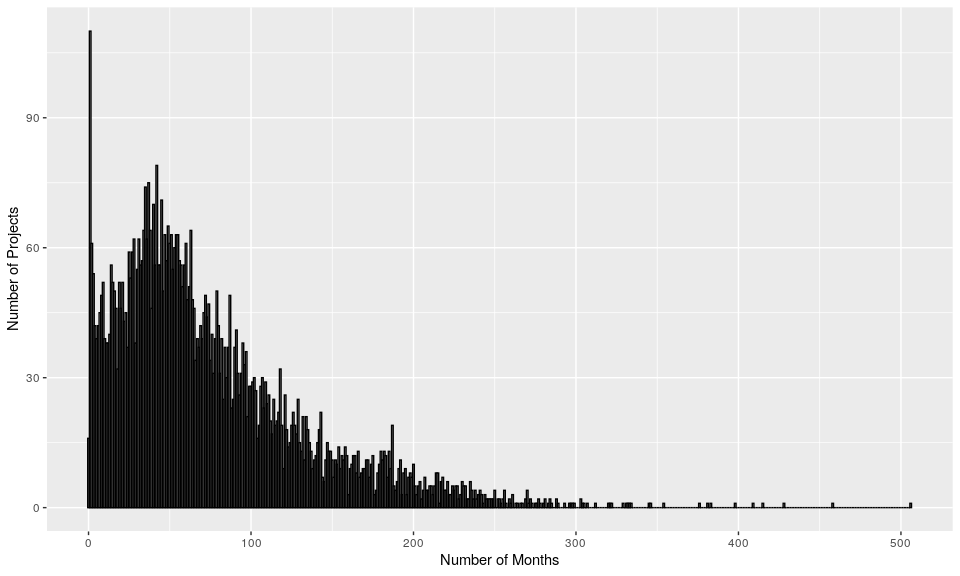
\includegraphics[width=\textwidth,keepaspectratio]{project-durations.png}
\end{frame}

\begin{frame}{World of Code Problems}
\begin{itemize}
    \item On two separate days, the sampling web application returned no results for any search. While we were able to get searches working on another day, we decided it was too unreliable to depend on.    
    \item It wasn't clear what was the best source of project data to select our sample of projects from.
    \item It took considerable time to determine that the Clickhouse database could not be used to get the commits per month time series data we needed.
    \item The commits data from the maps we have obtained is not consistent with the MongoDB data about each project. We're not sure yet if that's a problem with our scripts or an actual data inconsistency.
\end{itemize}
\end{frame}

\begin{frame}{Changepoint Detection}
We tested three techniques for changepoint detection on 
    \begin{itemize}
        \item Synthetic time series constructed with known changepoints.
        \item Commits time series for OpenSSL, where we know were changepoints exist from external events and prior analysis.
    \end{itemize}
The three techniques were
    \begin{itemize}
        \item Segmented regression, which always finds a changepoint.
        \item Changepoint detection (PELT).
        \item Nonparametric changepoint detection.
    \end{itemize}
\end{frame}

\begin{frame}{Projects by Number of Changepoints}
    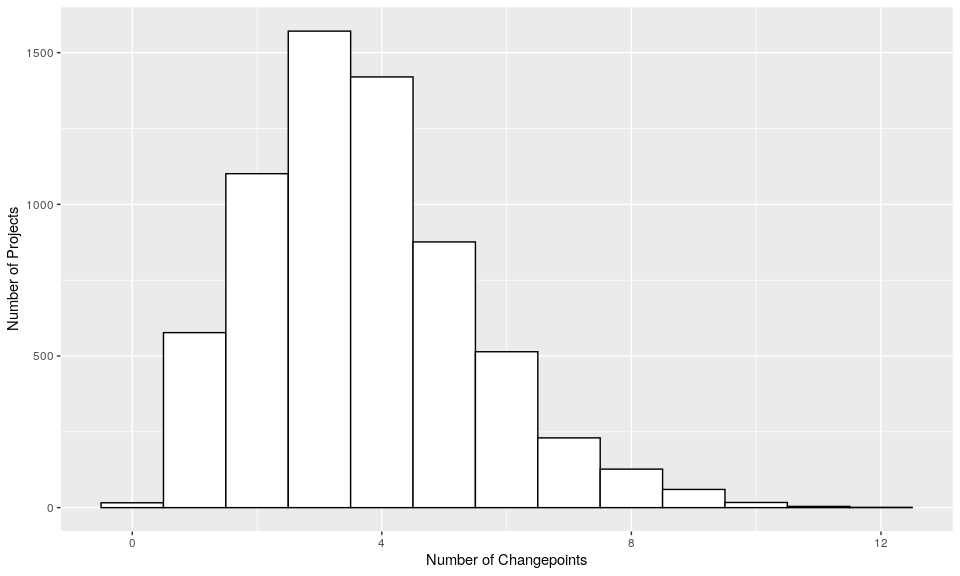
\includegraphics[width=\textwidth,keepaspectratio]{project-changepoints.png}
\end{frame}

\begin{frame}{Future Plans}
    \begin{enumerate}
        \item Identify and fix problems in data collection process.
        \item Tune algorithms and parameters for changepoint detection.
        \item Classify changepoints by size and magnitude.
        \item Collect unique authors and files changed time series data.
        \item Classify changepoints of new time series.
        \item Identify correlations in changepoints across different time series for the same project.
    \end{enumerate}
\end{frame}

\end{document}
